\documentclass[11pt,a4paper]{article}

% --- packages ---
\usepackage[a4paper, top=2cm, bottom=2cm, left=2cm, right=2cm]{geometry}
\usepackage[utf8]{inputenc}        % allow é, ï, etc.
\usepackage[T1]{fontenc}           % proper text encoding
\usepackage{tikz}                  % drawing the forest plot
\usepackage{xcolor}                % named colors
\usepackage{caption}               % \captionof{figure}{...}
\usepackage{booktabs}              % \toprule, \midrule, \bottomrule
\usepackage{graphicx}              % \includegraphics
\usepackage{eurosym}               % \euro{} for euro signs (we'll use later)
\usetikzlibrary{arrows.meta, positioning, fit}

% tighten paragraph spacing for the page budget
\setlength{\parskip}{4pt plus 1pt minus 1pt}
\setlength{\parindent}{0pt}

% figures generated by the notebook live here
\graphicspath{{reporting/figures/}}

% --- custom colors used in the figure ---
\definecolor{accent}{HTML}{2E5C8A}    % blue
\definecolor{accent2}{HTML}{4C9A4A}   % green (v3 — causally identified)
\definecolor{accent3}{HTML}{C04848}   % red (v1 — wrong sign)
\definecolor{accent4}{HTML}{E0B341}   % amber (v4, v5 — over-controlled)

\title{Dynamic Pricing for European Camping Group}
\author{Jimmy Zhang, Tobias Vanoverschelde, Fausto De Valck, Andrew Posey, 
Alexander Lievens \\ KU Leuven, Statistical Consulting 2025-2026, ORTEC Project}
\date{May 2026}

\begin{document}
\maketitle

\section{Problem and business context}

European Camping Group (ECG) operates over 400 campsites across 10 European countries, each offering several accommodation types and serving four distinct market segments. With a 30-week open season, this implies more than 250{,}000 individual prices to set every year, one for every combination of campsite, accommodation, market, and arrival-week. We refer to such a combination as a \emph{ROMGID} (reservable-option-market-group), the unit of analysis throughout the report. This project examines: can historical booking data be used to recommend better prices for these ROMGID's, and what would that be worth in revenue?

\section{The trap}

The most direct approach, regressing booked nights on price while controlling for accommodation and seasonality, yields an answer that is economically impossible. On a 50{,}000 row training sample, the estimated price coefficient is positive: $\beta = +0.29$, with the 80\% credible interval $[+0.18, +0.42]$. Read literally, this means ``raising prices increases bookings''.

The reason is structural, not statistical. ECG's pricing system already reacts to demand: when a campsite fills up, prices rise, when bookings are slow, prices fall. In the historical record, high prices and high bookings therefore tend to occur together, not because price causes bookings, but because both respond to a common, unobservable underlying demand signal.

The fix requires identifying the demand signal that the pricer reacts to. Bookings on books, the cumulative number of nights already reserved at the moment a price is set, is observed in our data and lies on the only open backdoor path between price and remaining demand. Conditioning on it blocks the reverse-causation channel and better isolates the genuine effect of price.

\begin{center}
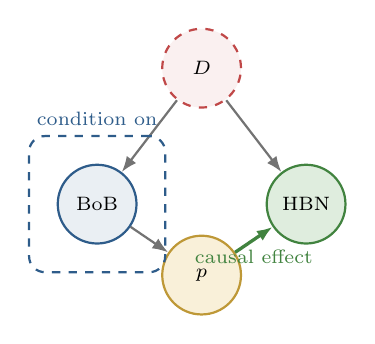
\begin{tikzpicture}[
  obs/.style={circle, draw=accent, thick, fill=accent!10, minimum size=10mm, font=\scriptsize, inner sep=0pt},
  latent/.style={circle, draw=accent3, thick, dashed, fill=accent3!8, minimum size=10mm, font=\scriptsize, inner sep=0pt},
  treatment/.style={circle, draw=accent4!85!black, thick, fill=accent4!20, minimum size=10mm, font=\scriptsize, inner sep=0pt},
  outcome/.style={circle, draw=accent2!85!black, thick, fill=accent2!18, minimum size=10mm, font=\scriptsize, inner sep=0pt},
  arrow/.style={-{Latex[length=2mm]}, thick, draw=black!55},
  causal/.style={-{Latex[length=2mm]}, thick, draw=accent2!85!black, line width=1.2pt},
]
\node[latent]    (D)                                       {$D$};
\node[obs]       (BoB) [below left=10mm and 6mm of D]      {BoB};
\node[treatment] (P)   [below=16mm of D]                   {$p$};
\node[outcome]   (Y)   [below right=10mm and 6mm of D]     {HBN};

\draw[arrow]  (D)   -- (BoB);
\draw[arrow]  (BoB) -- (P);
\draw[arrow]  (D)   -- (Y);
\draw[causal] (P)   -- (Y) node[midway, below, font=\scriptsize, color=accent2!85!black] {causal effect};

% Highlight that we condition on BoB
\node[draw=accent, thick, dashed, rounded corners=2mm, inner sep=3.5mm,
      fit=(BoB), label={[font=\scriptsize, color=accent]above:condition on}] {};
\end{tikzpicture}
\captionof{figure}{Causal structure linking price ($p$) and bookings (HBN). Latent demand $D$ (red, dashed, unobservable) drives bookings-on-books (BoB, observed) and bookings directly. The existing pricer sets $p$ in response to BoB. The path $p \leftarrow \mathrm{BoB} \leftarrow D \to \mathrm{HBN}$ is a backdoor: it lets demand contaminate the apparent price-bookings relationship. Conditioning on BoB (dashed blue box) closes it, leaving only the genuine causal effect $p \to \mathrm{HBN}$.}
\end{center}

\smallskip

\begin{center}
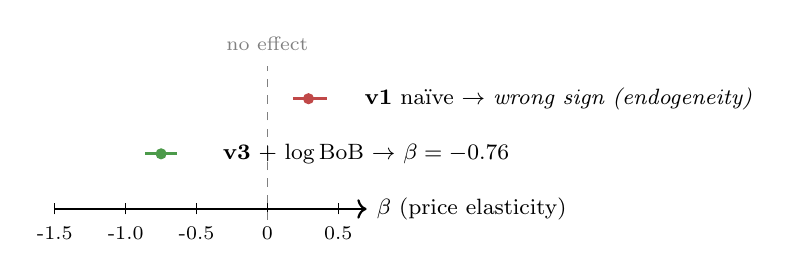
\begin{tikzpicture}[x=18mm, y=7mm]
  % axis (zoomed in to v1 / v3 range)
  \draw[->, thick] (-1.5, 0) -- (0.7, 0) node[right, font=\footnotesize] {$\beta$ (price elasticity)};
  \foreach \x in {-1.5, -1.0, -0.5, 0, 0.5} {
      \draw (\x, -0.1) -- (\x, 0.1);
      \node[below, font=\scriptsize] at (\x, -0.15) {\x};
  }
  \draw[dashed, gray] (0, -0.2) -- (0, 2.6);
  \node[gray, font=\scriptsize, above] at (0, 2.7) {no effect};

  % v1 — naïve, wrong sign
  \draw[thick, accent3, line width=1pt] (0.18, 2.0) -- (0.42, 2.0);
  \filldraw[accent3] (0.29, 2.0) circle (1.8pt);
  \node[right=3mm, font=\footnotesize] at (0.45, 2.0) {\textbf{v1} naïve $\to$ \emph{wrong sign (endogeneity)}};

  % v3 — conditioned on log_bob
  \draw[thick, accent2, line width=1pt] (-0.86, 1.0) -- (-0.64, 1.0);
  \filldraw[accent2] (-0.75, 1.0) circle (1.8pt);
  \node[right=3mm, font=\footnotesize] at (-0.55, 1.0) {\textbf{v3} $+\,\log\mathrm{BoB}$ $\to$ \emph{$\beta = -0.76$}};
\end{tikzpicture}
\captionof{figure}{Posterior point estimate and 80\% credible interval for the global price elasticity $\beta$. The naïve specification (v1) recovers an economically impossible positive sign, direct evidence of price endogeneity in ECG's data. After conditioning on bookings-on-books, the elasticity becomes negative as economic theory requires (v3, $\beta = -0.76$).}
\end{center}

\section{Two models, two jobs}

The Bayesian estimate of $\beta = -0.76$ from model v1 implies demand is inelastic on average ($|\beta| < 1$). In plain language, every 1\% price increase reduces bookings by about 0.76\%. Because the response is less than proportional, total revenue (price multiplied by bookings), on average, goes up when prices go up, at least within the price range our data cover. Under a constant-elasticity assumption, this would mean ECG could raise prices uniformly and capture more revenue. A richer LightGBM optimiser in Section 4 refines this picture: average elasticity is right, but per-cell optima vary widely. Some campsite-week cells are over-priced, others under-priced, and the aggregate move is close to zero. The business case for a pricing engine on this dataset is therefore not ``raise everything'' but ``identify the asymmetries'', figuring out which cells should move, in which direction, and by how much.

Model v3 is intentionally minimal: it only uses the variables strictly needed to close the backdoor. This makes it a clean estimator of the local average elasticity but not a forecaster. To predict bookings at any candidate price for any single snapshot of the booking horizon, we train a gradient-boosted-trees model (LightGBM) on the same conditioning structure plus the lead-time, calendar and accommodation features that v3 deliberately omits. Trees can include all of these without the over-conditioning collapse that breaks richer Bayesian specifications. At typical prices, the LightGBM model implies the same local price-bookings slope as the Bayesian model (around $-0.75$), a useful cross-check: two methods with very different assumptions arrive at the same answer.

Out-of-sample, LightGBM achieves a median ROMGID-level error of 27\% on total booked nights, within industry norms. The error is concentrated in low-volume ROMGID's where small absolute differences inflate percentage errors. For ROMGID's with at least 10 bookings per season, median error drops to 22\%.

\section{The optimiser and what it recommends}

For each test-fold snapshot independently, we ask the LightGBM forecaster a counterfactual question: at this point in the booking horizon, what price would have produced the highest predicted revenue? We sweep 21 candidate price multipliers in the range $[0.85,\, 1.15] \times p_{\mathrm{obs}}$, predict bookings at each candidate, compute the implied revenue $p \cdot \hat{N}(p)$, and pick the maximum. The output for a single ROMGID is therefore not a single static price but a trajectory of 53 prices across the booking horizon, one per snapshot.

Three constraints keep the recommendation defensible: the candidate range is capped at $\pm 15\%$ of historical prices for that group, predicted bookings are clipped at capacity, and every recommendation passes through a two-tier flag (green / yellow) before deployment, keeping the human in the loop.

\newpage Applied to 14{,}200 ROMGID's in the held-out test fold:

\begin{center}
\small
\begin{tabular}{@{}lr@{}}
\toprule
\textbf{Metric} & \textbf{Value} \\
\midrule
Median per-ROMGID $\Delta$price & $-0.7\%$ \\
$\Delta$price IQR (per ROMGID) & $[-6.0\%,\, +5.4\%]$ \\
\% snapshots at upper bound (1.15$\times$) & 12.7\% \\
\% snapshots at lower bound (0.85$\times$) & 14.7\% \\
\% snapshots with interior optimum & \textbf{72.6\%} \\
Total predicted uplift & \euro{}63M \\
Uplift as \% of baseline & $+38.8\%$ \\
Flag split (green / yellow) & 51\% / 49\% \\
\bottomrule
\end{tabular}
\end{center}

\begin{center}
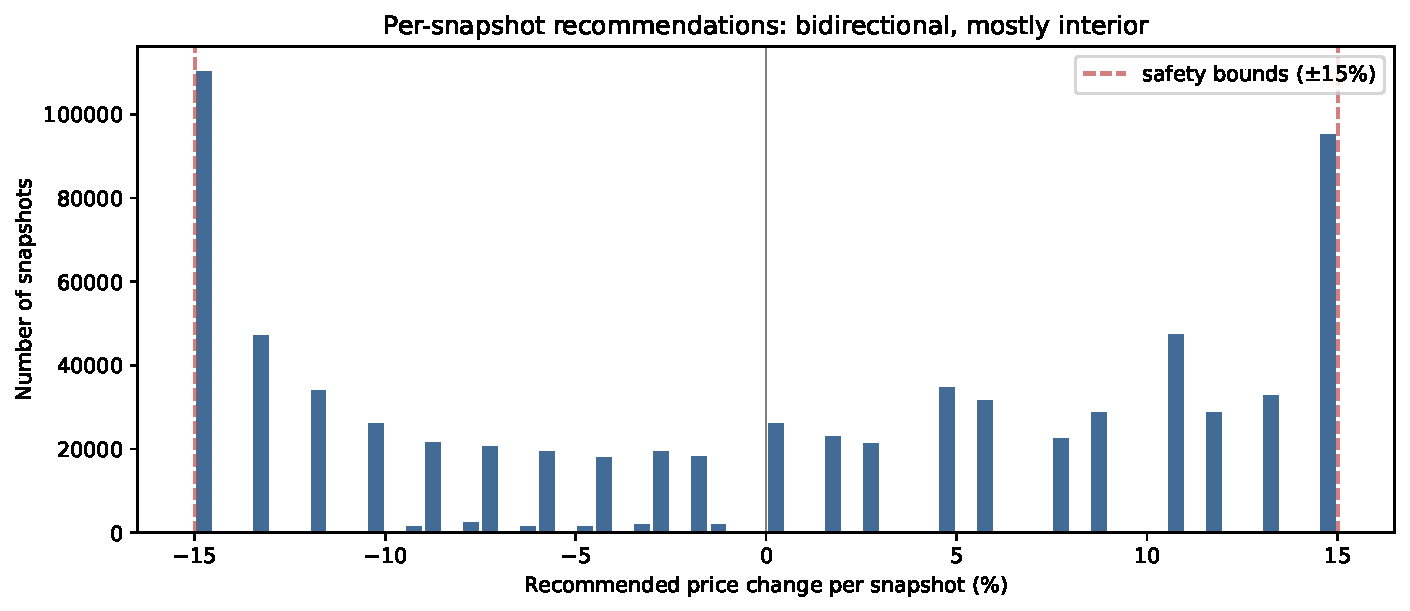
\includegraphics[width=0.7\linewidth]{recommendations_distribution.pdf}
\captionof{figure}{Distribution of recommended price changes across all test-fold snapshots. The histogram is roughly symmetric around zero, with mass at both the lower and upper safety bounds. About 73\% of decisions land at an interior optimum within the safe range, 14.7\% want a 15\% discount, and 12.7\% want a 15\% increase.}
\end{center}

The most important number on the page is the \textbf{72.6\% interior-optimum rate}. For nearly three quarters of snapshot decisions, the model finds a revenue-maximising price strictly inside the $\pm 15\%$ safe range, not at a boundary. This is something the constant-elasticity Bayesian model in Section 2 could not produce. When elasticity is forced constant the revenue function has no interior maximum, but when LightGBM learns a flexible price-demand curve, genuine interior optima emerge. The recommendations are also bidirectional, 14.7\% of snapshots want a price decrease and 12.7\% want the maximum 15\% increase. ECG is over-pricing some cells and under-pricing others, with the bulk of decisions sitting at modest interior adjustments.

\begin{center}
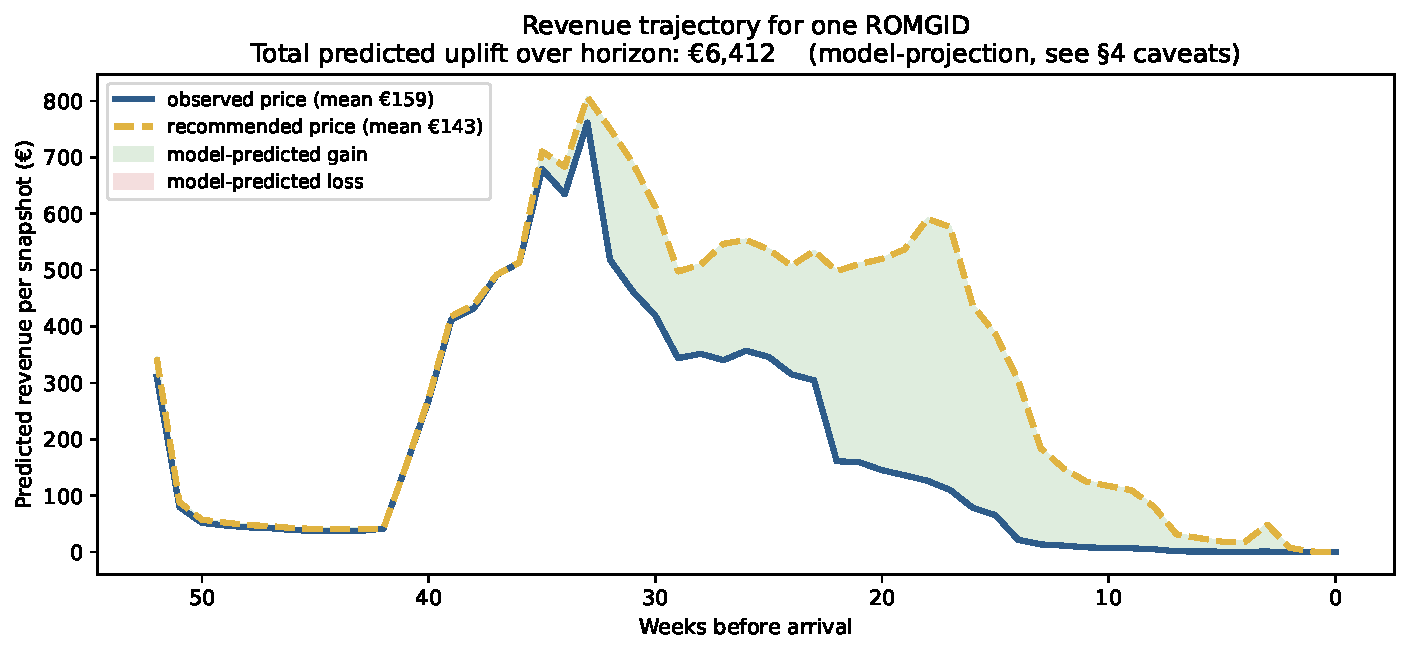
\includegraphics[width=0.7\linewidth]{revenue_trajectory.pdf}
\captionof{figure}{Predicted revenue per snapshot for one representative ROMGID, observed price (blue) versus recommended price (amber), with 80\% prediction intervals from a quantile LightGBM. Most of the booking horizon shows similar predicted revenue under both strategies, with the recommended trajectory slightly higher in the mid-horizon weeks where bookings actually concentrate.}
\end{center}

The +\euro{}63M total predicted uplift is a model projection and is almost certainly optimistic, for three reasons. First, the model has 27\% out-of-sample error on observed prices, and counterfactual prices push it further from familiar ground. Second, the optimiser picks the candidate that maximises predicted revenue, exploiting any residual model error in its own favour. Third, the model can predict small positive bookings even in late-horizon snapshots where actual bookings are essentially zero, and the optimiser sees these as small revenue gains. The directional finding (interior optima, modest adjustments, bidirectional recommendations) is robust, but the magnitude is not. A randomised price experiment, discussed next, is the only way to convert it into a number ECG can budget against.

\section{What ECG should do next}
 
The pipeline already produces a \texttt{recommendations.csv} every time it
runs, with one row per ROMGID containing the current price, the recommended
price, predicted bookings, revenue uplift with an 80\% credible interval, and
a human-in-the-loop flag. Because the model conditions on bookings-on-books at
the moment of prediction, any new reservation that enters ECG's booking system
automatically shifts the ROMGID to a different point on the demand curve the
model has already learned. A nightly batch job recomputes features for all
active ROMGID's, reruns the price sweep, and regenerates the file, so a
dashboard could always reflect the most recent booking state without requiring model
retraining. Retraining itself could happen once per season, when a full new round of
observations is available to update the elasticity estimates. This file is
designed to feed a pricing dashboard that can be embedded directly into ECG's
existing revenue-management workflow.
 
The prototype dashboard we deliver alongside this report reads the recommendation file and presents each ROMGID as a row in a sortable, filterable table.  A pricing
manager opening this dashboard in the morning sees, for every campsite--week
combination, the current price next to the model's recommended price, the
percentage change, the predicted revenue uplift, and a colour-coded flag.
Clicking a row expands a detail panel with the full context: observed versus
predicted bookings, a capacity-utilisation bar, historical price volatility,
and a plain-language explanation of why this particular recommendation was
flagged the way it was.

\begin{center}
\small
\begin{tabular}{@{}llllrrr@{}}
\toprule
\textbf{ROMGID} & \textbf{Campsite} & \textbf{Type} & \textbf{Flag} & \textbf{Current} & \textbf{Recommended} & \textbf{$\Delta$price} \\
\midrule
0042 & CS-FR-118 & Mobile Home & \colorbox{accent4!25}{yellow} & \euro{}187 & \euro{}164 & $-12.3\%$ \\
\bottomrule
\end{tabular}
\captionof{figure}{Example row from the pricing dashboard. This ROMGID is flagged yellow because the recommended adjustment exceeds 10\%; the pricing manager reviews local context before approving.}
\end{center}
 
The flag system is the mechanism that connects the model to the human.  A
\textbf{green} flag means the recommended adjustment is small (at most 10\%
change) and the historical price for this ROMGID has been stable (coefficient
of variation below 0.15).  The model is confident and the baseline is reliable;
once trust has been established through shadow-mode validation, green
recommendations could be auto-applied.  A \textbf{yellow} flag means either the
adjustment is larger (10--20\%) or the historical price has been moderately
volatile; the model's recommendation is plausible but needs a human to check
what the model cannot see: a local festival, an incoming weather front, a
competitor's flash sale.  These recommendations appear as the manager's daily
review queue.
 
More concretely, in the first season (shadow mode), no prices change: the
model generates recommendations, the dashboard displays them, and managers
compare the model's suggestions against their own decisions after the fact.
This builds an empirical track record: for which ROMGID's the model would
have done better, and for which it would have done worse, and lets the team
calibrate their trust before any automation.  In the second season, green-flag
recommendations that performed well in shadow mode can be auto-applied, while
yellow and red flags remain in the review queue.  The manager's role shifts
from setting every price to auditing the exceptions, which is a more efficient
use of their domain knowledge. 
 
\section{Conclusion}
 
Treating dynamic pricing as a causal-inference problem reveals a clear
endogeneity trap and a defensible local elasticity of $-0.76$ once it is
closed.  A complementary LightGBM forecaster delivers per-snapshot
recommendations that are differentiated and bidirectional, identifying which
cells should move and in which direction.  The outcome is not just a model
but a working pipeline: a recommendation file, a flag-based review workflow
embedded in a dashboard, and a phased integration plan that starts with shadow
mode and moves toward selective automation.  The engine does not replace the
pricing manager; it focuses their attention on the ROMGID's where intervention
matters most, while automating the large share of stable, low-risk decisions. This aspect is also important in convincing the existing managers to adopt this new project and in not neglecting their existing expertise by overruling their judgement entirely.
 
ECG's status quo is likely leaving model-identifiable revenue on the table.
The size of that revenue is the open question this report cannot answer alone,
but a small randomised experiment is designed to answer it within one season,
at negligible cost


\end{document}
